\documentclass[a4paper,10pt]{article}

% Hier die Nummer des Blatts und Autoren angeben.
\newcommand{\blatt}{9}
\newcommand{\autor}{Ralf Engelken, Joachim Schmidberger, Frank Woithe, Michael Steinke, Merlin Koglin}

\usepackage{hci}
\usepackage{float} 

\begin{document}
% Seitenkopf mit Informationen
\kopf
\renewcommand{\figurename}{Figure}

\aufgabe{14 \textit{(Team-Aufgabe)}} 

Sie sollen für eine von Ihnen entwickelte beliebige App ein neues Icon designen. Das bisherige Icon zeigt eine sehr realistische Darstellung der Bildelemente. Das neue Icon soll im Stil „Flat-Design“ gestaltet werden. Ihr Icon soll passende Elemente (wie beispielsweise Wolken, Sonne und Himmel für eine Wetter-App) beinhalten.

a) Erarbeiten Sie sich zunächst mit Hilfe diverser Sketches verschiedene Ideen, wie Ihr Icon aussehen soll. Diskutieren Sie zwischendurch immer wieder die unterschiedlichen Ansätze in der Gruppe.

b) Wenn Sie sich für ein grobes Layout entschieden haben, verfeinern Sie Ihre Illustrationen und fertigen einen ersten Papier-Prototypen an, bei dem Sie bereits deutlich machen, welche Gestaltprinzipien (Goldener Schnitt, Farbharmonien, Goldene Spirale etc.) Sie planen anzuwenden.

c) Verwenden Sie ein vektorbasierte Grafikprogramm Ihrer Wahl (Illustrator, Inkscape), um Ihr Icon umzusetzen.

d) Beschreiben Sie Ihr Icon, wobei Sie jede Design-Entscheidung dokumentieren. Begründen Sie auch Abstände, Formen und Farben.

Laden Sie Ihre Bearbeitung als PDF Datei (inklusive Sketches, Grafiken, Icon, Screen-Mockups und Beschreibung) sowie zusätzlich das Icon als SVG bis zum 20.6.2016 um 12 Uhr hoch.\\
\newpage
 
\textbf{\textit{Icon für eine Bilbiotheks App)}} \newline
Zunächst haben wir in ein paar schnellen Skaches die Ideen Festgehalten. Beim Thema Biblieothek war natürlich naheliegend, Bücher als Metapher zu wählen.
\begin{figure}[H]
\centering 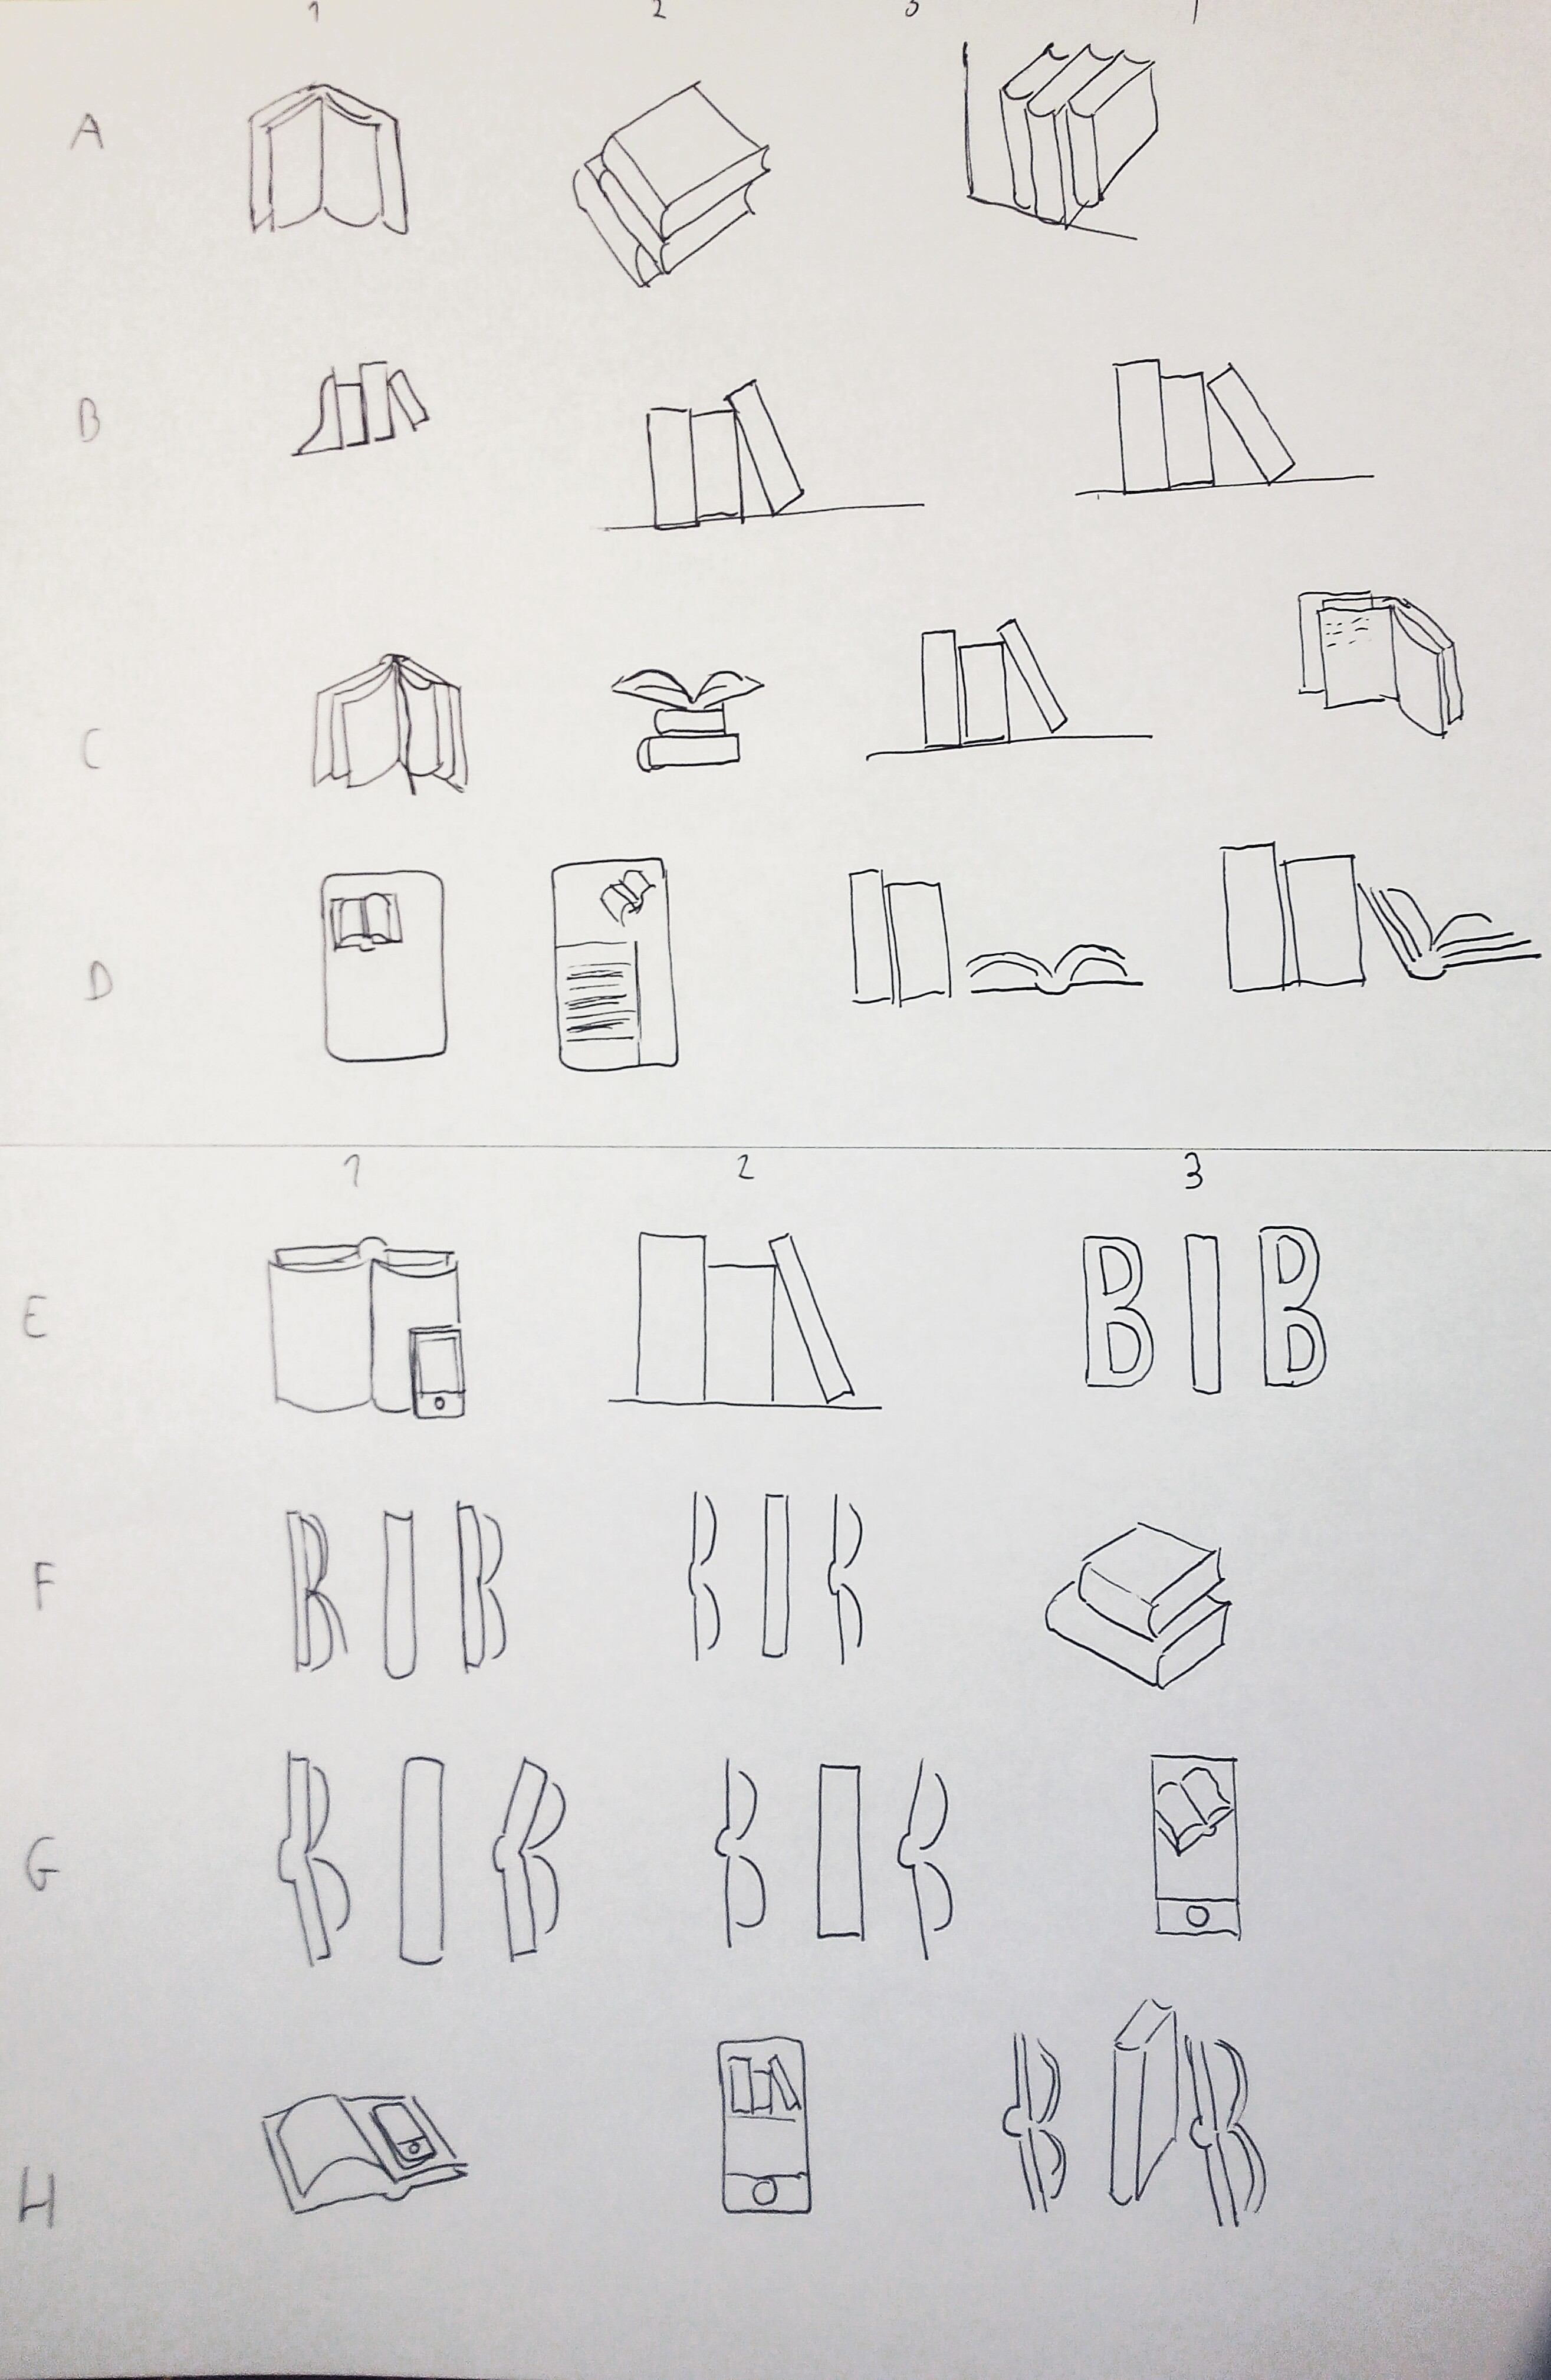
\includegraphics[width=0.8\textwidth]{sketches}
\caption{Ein paar schnelle Sketches}
\end{figure}

\textbf{\textit{Designentscheidung: Bücher als Buchstaben}} \newline
Die Idee Bücher als Buchstaben zu verwenden wurde als Interessant genug erachtet um weiter verfolgt zu werden. Die \textit{Buch - Staben} sollten gleichzeitig die Abkürzung \textit{Bib} bilden, wie sie oft für Bibliotheken umgangssprachlich verwendet wird. 
\begin{figure}[ht]
\centering 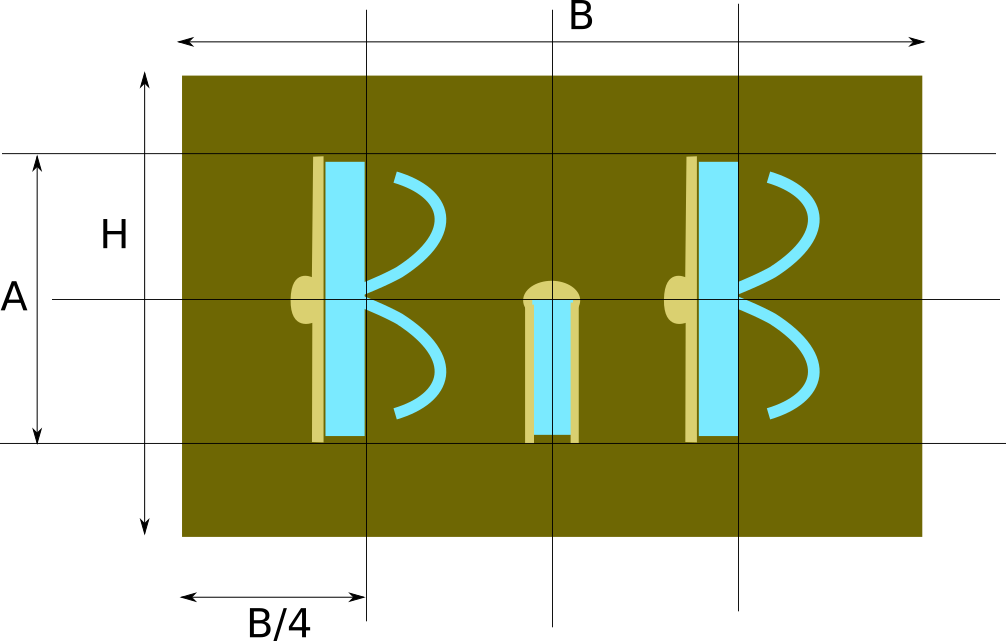
\includegraphics[width=0.8\textwidth]{bib_konst}
\caption{Ikon mit Hilfslinien}
\end{figure}
\newpage
\textbf{\textit{Bücher als Buchstaben im Flat-Design}} \newline
Das äussere Format des Ikons richtet sich nach dem Goldenen Schnitt. Es ist ca. 1,6 mal so breit wie hoch. Die senkrechten Hilfslinien teilen das Ikon in 4 Spalten, an denen sich die 3 Buchstaben orientieren. Die höhe der Buchstaben im Verältnis zur Gesammthöhe entspricht wiederum dem goldenen Schnitt.\\
Die Farben Des Ikons wurden entsprechend des Flat-Design Stils als leuchtend aufgehellte Mischfarben gewählt. Durch den dunkleren Hintergrund wird das Leuchten der Buchstaben-Bücher noch unterstrichen.
\begin{figure}[ht]
\centering \includegraphics[width=0.8\textwidth]{bib5}
\caption{Das Bibliothek-App Ikon}
\end{figure}
\end{document}
